\documentclass[10pt]{article}
\usepackage{fullpage}
\usepackage{bnf}
\usepackage{graphicx}
\usepackage{listings,color,xcolor}
\usepackage{caption}
\usepackage{listings}
\usepackage{gantt}
\usepackage{tikz}
\usepackage{longtable}
\usepackage[bookmarks]{hyperref}
\usepackage{url}
\usetikzlibrary{arrows}

\newcommand{\Lang}{GAMMA}
\newcommand{\Compiler}{ray}

\renewcommand{\lstlistingname}{Example}
\renewcommand{\lstlistlistingname}{Examples}

\setlength{\parskip}{4pt}

\definecolor{tintedgray}{rgb}{0.96,0.96,0.96}
\definecolor{tintedorange}{rgb}{1,0.96,0.9}

\lstdefinestyle{example_style}{ %
  aboveskip=8pt,
  abovecaptionskip=8pt,
  backgroundcolor=\color{tintedgray},
  basicstyle=\footnotesize,
  belowskip=0pt,
  breakatwhitespace=false,
  breaklines=true,
  captionpos=b,
  commentstyle=\color{orange},
  frame=single,
  framesep=8pt,
  float,
  keepspaces=true,
  keywordstyle=\color{blue},
  morekeywords={and,class,else,elsif,extends,false,
  	if,init,main,nand,new,nor,not,null,or,private,
  	protected,public,refinable,refine,refinement,
  	return,super,this,to,true,void,while,xor},           
  numbers=left,
  numbersep=14pt,
  numberstyle=\tiny\color{gray},
  rulecolor=\color{black},
  showspaces=false,
  showstringspaces=false,
  showtabs=false,
  stepnumber=1,
  tabsize=4,
  title=\lstname
}
\lstset{style=example_style}

\title{\Lang{}: A Strict yet Fair Programming Language}
\author{
	Ben Caimano - blc2129@columbia.edu \\
	Weiyuan Li - wl2453@columbia.edu \\
	Matthew H Maycock - mhm2159@columbia.edu \\
	Arthy Padma Anandhi Sundaram - as4304@columbia.edu
}
\date{}

\begin{document}
\noindent
\includegraphics[width=\textwidth]{logo.png}
\pagebreak

%Title area
\maketitle
\begin{center}
\large
A Project for Programming Languages and Translators,
\\taught by Stephen Edwards
\end{center}

%Introduction
\section{Introduction}
\subsection{Why \Lang{}? -- The Core Concept}
We propose to implement an elegant yet secure general purpose object-oriented programming language. Interesting features have been selected from the history of object-oriented programming and will be combined with the familiar ideas and style of modern languages.

\Lang{} combines three disparate but equally important tenants:


\begin{enumerate}
\item Purely object-oriented 
    
    \Lang{} brings to the table a purely object oriented programming language where every type is
    modeled as an object--including the standard primitives. Integers, Strings, Arrays, and other types may be expressed in the standard fashion but are objects behind the scenes and can be treated as such.

\item Controllable

   \Lang{} provides innate security by choosing object level access
   control as opposed to class level access specifiers. Private members of one object
   are inaccessible to other objects of the same type. Overriding is not allowed.
   No subclass can turn your functionality on its head.

\item Versatile

    \Lang{} allows programmers to place "refinement methods" inside their code.
    Alone these methods do nothing, but may be defined by subclasses so as to extend
    functionality at certain important positions. Anonymous instantiation allows for
    extension of your classes in a quick easy fashion.
\end{enumerate}

\subsection{The Motivation Behind \Lang{}}
\Lang{} is a reaction to the object-oriented languages before it.
Obtuse syntax, flaws in security, and awkward implementations plague
the average object-oriented language. \Lang{} is intended as a step
toward ease and comfort as an object-oriented programmer.


The first goal is to make an object-oriented language that is comfortable
in its own skin. It should naturally lend itself to constructing API-layers
and abstracting general models. It should serve the programmer towards their
goal instead of exerting unnecessary effort through verbosity and awkwardness
of structure.


The second goal is to make a language that is stable and controllable.
The programmer in the lowest abstraction layer has control over how those
higher may procede. Unexpected runtime behavior should be reduced through
firmness of semantic structure and debugging should be a straight-forward
process due to pure object and method nature of \Lang{}.


\pagebreak

\tableofcontents

\section{Language Tutorial}

The structure of the example below should be intimately familiar to any student of Object-Oriented Programming. 
\lstinputlisting[caption="A simple I/O example"]{../../ray/compiler-tests/programs/io.gamma}

We start with a definition of our class.

\begin{lstlisting}
class IOTest:
\end{lstlisting}

We follow by starting a \verb!public! access level, defining an \verb!init! method for our class, and calling the \verb!super! method inside the init method. (Since we have not indicated a superclass for \verb!IOTest!, this \verb!super! method is for \verb!Object!.)

\begin{lstlisting}
    public:
        init():
            super()
\end{lstlisting}

We also define the \verb!private! access level with three methods: a generic method that prints a prompt message and two prompts for \verb!Integers! and \verb!Floats! respectively. These prompts call the generic message and then read from \verb!system.in!.

\begin{lstlisting}
  private:
    void prompt(String msg):
      system.out.printString(msg)
      system.out.printString(": ")

    Integer promptInteger(String msg):
      prompt(msg)
      return system.in.scanInteger()

    Float promptFloat(String msg):
      prompt(msg)
      return system.in.scanFloat()
\end{lstlisting}

We then write a method under the \verb!public! access level. This calls our \verb!private! level methods, convert our \verb!Integer! to a \verb!Float! and print our operation.

\begin{lstlisting}
    void interact():
      Printer p := system.out
      Integer i := promptInteger("Please enter an integer")
      Float f := promptFloat("Please enter a float")
      p.printString("Sum of integer + float = ")
      p.printFloat(i.toF() + f)
      p.printString("\n")
\end{lstlisting}

Finally, we define the \verb!main! method for our class. We just make a new object of our class in that method and call our sole public method on it.


\begin{lstlisting}
  main(System system, String[] args):
    IOTest test := new IOTest()
    test.interact()
\end{lstlisting}

\section{Language Reference Manual}
\section{Lexical Elements}
\subsection{Identifiers}
Identifiers are used for the identification of variable,  methods and types. An identifer is a sequence of alphanumeric characters, uppercase and lowercase, and underscores. A variable or method identifier must start with a lowercase alphabetic character. A type identifier must start with an uppercase alphabetic character.

\subsection{Keywords}
The following words are reserved keywords. They may not be used as identifiers:
\begin{center}
\begin{tabular}{ccccccc}
and & class & else & elsif & extends & extends & false\\
if & init & nand & new & nor & null & or\\
private & protected & public & refinable & refine & refinement & return\\
super & this & to & true & while & void & xor\\
\end{tabular}
\end{center}

\section{Semantics}

\subsection{Types and Variables}
Every \textit{variable} in Gamma is declared with a \textit{type} and an \textit{identifier}. The typing is static and will always be known at compile time for every variable. The variable itself holds a reference to an instance of that type. At compile time, each new instantiation reserves space for one instance of that type. To be an instance of a type, an instance must be an instance of the class of the same name as that type, an instance of one of the set of descendants (i.e. a subclass defined via \verb!extends!) of that class, or the {\tt null} instance. For the purposes of function declaration, there is a special type, \textit{Void}, that allows a function to use the \verb!return! keyword without an expression.

\subsubsection{Arrays}
When specifying a type, the type can be suffixed with square brackets to indicate that it instead an array of that type. The individual instances of the array can be accesed by using the variable identifier with an index. --- I'm just not sure how to do this.

\subsection{Classes, Subclasses and Their Members}
\Lang{} is a pure object-oriented language, which means every value is an object--with the exception of the reserved references \verb!null! and \verb!this!. A class always extends another class; a class inherits all of its superclass's methods and may refine the methods of its superclass. A class must contain a constructor routine named {\tt init} and it must invoke its superclass's constructor via the super keyword -- either directly or transitively by referring to other constructors within the class. In the scope of every class, the keyword \verb!this! explicitly refers to the instance itself. Additionally, a class contains three sets of \textit{members} organized in \textit{private}, \textit{protected}, and \textit{public} sections. Members may be either variables or methods. Each class must be derived from another class as a \textit{subclass}.

\subsubsection{The Object Class}
The Object class is the superclass of the entire class hierarchy in \Lang{}. All objects directly or indirectly inherit from it and share its methods. By default, class declarations without extending explicitly are subclasses of Object.

\subsubsection{The Literal Classes}
There are several \textit{literal classes} that contain unique members that hold strictly data. These classes generally have methods developed for most operators. They are also all subclasses of Object.

\subsection{Methods}
A method is a reusable subdivision of code that takes multiple instances as arguments and returns either a variable of the type specified for the method or null. Methods of a class can have \textit{refine} statements placed in their bodies. Then subclasses must implement \textit{refinements}, special methods that are called in place of their superclass' refine statements. Optionally, the superclass can conditionally check if the refinement has been implemented to avoid runtime errors via the \verb!refinable! test.

\subsubsection{Operators}
Since all variables are classes, every operator is in truth a method called from the most precident opperand with the less precident opperand as an argument. If an operator is not usable with a certain literal class, then it will not have the method implemented as a member. Classes that are not literal classes may implement those functions so as to allow that operation to be performed between two instances of the appropriate type.

\subsection{Expressions and Statements}
The fundamental nature of an expression is that it generates a single instance. This instance may be in the form of a variable or the return value of a method. Note that the method could be in the form of an operator. If the expression is a method or operator, its arguments are, of course, other expressions. A statement can be a call to an expression, thus a method or a variable.


\section{Syntax}
\subsection{Variable Initialization}
Initializing a variable requires a type and a list of identifiers deliminated by commas:

\begin{lstlisting}
type identifier[, identifier[, identifier[...]]];
\end{lstlisting}

If we wanted to initialize variables for the pythagorean theorem, we would do it like so:

\begin{lstlisting}[caption=Variable Initialization for the Pythagorean Theorem]
Float a, b, c;
\end{lstlisting}

\subsection{Variable Assignment}
Assigning an instance to a variable requires an expression and a variable identifier:

\begin{lstlisting}
identifier := expression;
\end{lstlisting}

If we wanted to assign instances of Integer for our pythagorean theorem, we'd do it like so:

\begin{lstlisting}[caption=Variable Assignment for the Pythagorean Theorem]
a := 3;
b := 4;
\end{lstlisting}

\subsection{Method Invocation}
Invoking a method requires at least an identifier for the method of the current context (i.e. implicit \verb!this! receiver). The instance that the method is invoked upon can be provided as a variable. If it is not provided, the method is invoked upon the global state.

\begin{lstlisting}
[expression.]identifier([expression[, expression[...]]])
\end{lstlisting}

Finishing our pythagorean example, we use method invocations and assignment to calculate the length of our third side, c.

\begin{lstlisting}[label=Method Invocation,caption=Method Invocation for the Pythagorean Theorem Using Methods]
c := ((a.power(2)).plus(b.power(2))).power(0.5);
\end{lstlisting}

\subsection{Method Invocation Using Operators}
Alternatively, certain base methods allow for the use of more familiar binary operators in place of a method invocation.

\begin{lstlisting}
expression operator expression
\end{lstlisting}

Using operators has advantages in clarity and succinctness even if the end result is the same.

\begin{lstlisting}[label=Method Invocation,caption=Method Invocation for the Pythagorean Theorem Using Operators]
c := ( a^2 + b^2 )^0.5;
\end{lstlisting}

\subsection{Operator Precidence}
In the previous examples, parentheses were used heavily in a context not directly related to method invocation. Parentheses have one additional function: they modify precedence among operators. Every operator has a precidence in relation to its fellow operators. Operators of higher precidence are enacted first. Please consider the following table for determining precidence:
\begin{table}[h]\footnotesize
\begin{tabular}{ccccccc}
\verb!:=! & \verb!+=! & \verb!-=! & \verb!*=! & \verb!/=! & \verb!%=! & \verb!^=!\\
or & xor & nor &&&&\\
and & nand &&&&&\\
\verb!=! & \verb!<>! & \verb!=/=! &&&&\\
\verb!>! & \verb!<! & \verb!>=! & \verb!<=! &&&\\
\verb!+! & \verb!-! &&&&&\\
\verb!*! & \verb!/! & \verb!%! &&&&\\
not & \verb!^! &&&&&\\
\verb!(! & \verb!)! &&&&&\\
\multicolumn{3}{c}{array dereferencing}&&&&\\
\multicolumn{3}{c}{method invocation}&&&&\\
\end{tabular}
\caption{Operator Precidence}
\end{table}

\subsection{Method Declaration}
A method definition begins with either a return type or Void. The identifier for the function is followed by a pair of parentheses that may enclose the argument variable definitions. There is one type and one identifier for each argument; and they are delimited by commas. Following the parentheses are a pair of braces around the body of the method. In the body, there must be at least one statement but there may be many more. At least one of those statements must be a return statement. Additionally, refinements may be placed throughout the statements.
 
\begin{lstlisting}
return_type | Void method_identifier ([var_type var_identifier[, var_type var_identifier[, var_type var_identifier[...]]]]){
	statement*
	[statement*]
	[statement*]
	...
}
\end{lstlisting}

Finally, we may define a method to do our pythagorean theorem calculation.

\begin{lstlisting}[label=Method Invocation,caption=Method Definition for the Pythagorean Theorem]
Float pythagorean_theorem(Float a, Float b){
	c := ( a^2 + b^2 )^0.5;
	return c;
}
\end{lstlisting}

\subsection{Class Declaration}
A class definition always starts with the keyword \verb!class! followed by an identifier. It optionally has the keyword \verb!extends! followed by the identifier of the superclass. What follows is the class body in brackets: an optional \verb!main! method and the three access-level member sections. There may be \verb!init! methods in any of the three sections.

\begin{lstlisting}
class class_identifier [extends superclass_identifier]{
	init_method
	[main_method]
	[private{
		[private_method_decl | private_var_decl]
		[private_method_decl | private_var_decl]
		...
	}]
	[protected{
		[protected_method_decl | protected_var_decl]
		[protected_method_decl | protected_var_decl]
		...
	}]
	[public {
		[public_method_decl | public_var_decl]
		[public_method_decl | public_var_decl]
		...
	}]
	[refinement {
		[refinement_decl]
		[refinement_decl]
		...
	}]
}
\end{lstlisting}

Let's make a basic geometric shape class in anticipation of later examples. We have private members, two access-level sections and an init method. No extends is specified, so it is assumed to inherit from Object.


\begin{lstlisting}[label=Method Invocation,caption=Class Declaration for a Geometric Shape class]
class Geometric_Shape{
	private{
		String name;
		Float area;
		Float circumfrence;
	}
	public{
	    init (String name){
	    	    this.name = name;
	    	    if(refinable(improve_name)){
	    	    		this.name += refine(improve_name to String)
	    	    	} 
	    	    	return
	    }
	    Float get_area(){
	    		Float area;
	    		area := refine(custom_area to Float)
	    }
	}
}
\end{lstlisting}

\subsection{Class Instantiation}
Making a new instance of a class is simple.

\begin{lstlisting}
new class_identifier([expr[,expre[,expr[...]]]])
\end{lstlisting}

For instance:

\begin{lstlisting}[label=Method Invocation,caption=Class Instantiation for a Geometric Shape class]
Geometric_Shape = new Geometric_Shape("circle");
\end{lstlisting}

Note: If literal classes are always objects, can you use the \verb!new! construct with them? The answer has to be no. It conveys no benefit even if it was usable.

\subsection{Array Initialization}
Initializing an array is almost the same as initializing a normal variable, simply add square brackets after the type.

\begin{lstlisting}
type[] identifier[, identifier[, identifier[...]]];
\end{lstlisting}

\subsection{Conditional Structures}

\subsection{Refinements}

\section{Operators and Literal Types}
The following defines the approved behaviour for each combination of operator and literal type. If the literal type is not listed for a certain operator, the operator's behaviour for the literal is undefined. These operators never take operands of different types.
\subsection{The Operator \verb!=!}
\subsubsection{Integer}
If two Integer instances have the same value, \verb!=! returns \verb!true!. If they do not have the same value, it returns \verb!false!.
\subsubsection{Float}
If two Float instances have an absolute difference of less than or equal to an epsilon of 2^{-24}, \verb!=! returns \verb!true!. If the absolute difference is greater than that epsilon, it returns \verb!false!.
\subsubsection{Boolean}
If two Boolean instances have the same keyword, either \verb!true! or \verb!false!, \verb!=! returns \verb!true!. If their keyword differs, it returns \verb!false!.
\subsubsection{String}
If two String instances have the same sequence of characters, \verb!=! returns \verb!true!. If their sequence of characters differs, it returns \verb!false!.

\subsection{The Operators \verb!=/=! and \verb!<>!}
\subsubsection{Integer}
If two Integer instances have a different value, \verb!=/=! and \verb!<>! return \verb!true!. If they do have the same value, they returns \verb!false!.
\subsubsection{Float}
If two Float instances have an absolute difference of greater than than an epsilon of 2^{-24}, \verb!=! returns \verb!true!. If the absolute difference is less than or equal to that epsilon, it returns \verb!false!.
\subsubsection{Boolean}
If two Boolean instances have different keywords, \verb!=/=! and \verb!<>! return \verb!true!. If their keywords are the same, they return \verb!false!.
\subsubsection{String}
If two String instances have the different sequences of characters, \verb!=/=! and \verb!<>! return \verb!true!. If their sequence of characters is the same, they return \verb!false!.

\subsection{The Operator \verb!<!}
\subsubsection{Integer and float}
If the left operand is less than the right operand, \verb!<! returns \verb!true!. If the right operand is less than or equal to the left operand, it returns \verb!false!.
\subsubsection{String}
If the left operand comes before the right operand in dictionary order, \verb!<! returns \verb!true!. If the left operand comes after the right operand in dictionary order , it returns \verb!false!. If the two operands have the same sequence of characters, it returns \verb!false!.

\subsection{The Operator \verb!>!}
\subsubsection{Integer and float}
If the left operand is greater than the right operand, \verb!>! returns \verb!true!. If the right operand is greater than or equal to the left operand, it returns \verb!false!.
\subsubsection{String}
If the left operand comes after the right operand in dictionary order, \verb!<! returns \verb!true!. If the left operand comes before the right operand in dictionary order , it returns \verb!false!. If the two operands have the same sequence of characters, it returns \verb!false!.

\subsection{The Operator \verb!<=!}
\subsubsection{Integer and float}
If the left operand is less than or equal to the right operand, \verb!<! returns \verb!true!. If the right operand is less than the left operand, it returns \verb!false!.
\subsubsection{String}
If the left operand comes before the right operand in dictionary order, \verb!<! returns \verb!true!. If the left operand comes after the right operand in dictionary order , it returns \verb!false!. If the two operands have the same sequence of characters, it returns \verb!true!.

\subsection{The Operator \verb!>=!}
\subsubsection{Integer and float}
If the left operand is greater than or equal to the right operand, \verb!>! returns \verb!true!. If the right operand is greater than the left operand, it returns \verb!false!.
\subsubsection{String}
If the left operand comes after the right operand in dictionary order, \verb!<! returns \verb!true!. If the left operand comes before the right operand in dictionary order , it returns \verb!false!. If the two operands have the same sequence of characters, it returns \verb!true!.

\newcommand{\comment}[1]{{\escapegrammar$\bullet$\it\ #1}\\}

\section{Grammar}

\begin{grammar}
      [(colon){$\hskip 0.1cm \Rightarrow$\\$~\hskip 0.75cm$}]
      [(semicolon){\\$~\hskip 0.45cm|\hskip 0.2cm$}]
      [(comma){}]
      [(period){\\}]
      [(quote){\begin{bf}}{\end{bf}}]
      [(nonterminal){$\langle$}{$\rangle$}]

\comment{Classs may extend another class or default to extending Object}
<class>:"class ",<class id>,<extend>," \{ ",<class section>,"{\small *} \}".
<extend>:"$\epsilon$";"extends ",<class id>.

\comment{Sections -- private protected public refinements and main}
<class section>:<refinement>;<access group>;<main>.

\comment{Refinements are named method dot refinement}
<refinement>:"refinement \{ ",<refine>,"{\small *} \}".
<refine>:<return type>,<var id>,".",<var id>,<params>," \{ ",<statement>,"{\small *} \}".

\comment{Access groups contain all the members of a class}
<access group>:<access type>," \{ ",<member>,"{\small *} \}".
<access type>:"private";"protected";"public".
<member>:<var decl>;<method>;<init>.
<method>:<return type>,<var id>,<params>," \{ ",<statement>,"{\small *} \}".
<init>:"init ",<params>," \{ ",<statement>,"{\small *} \}".

\comment{Main is special -- not instance data, starts execution}
<main>:"main ( String[] ",<var id>," ) \{ ",<statement>,"{\small *} \}".

\comment{Finally, the meat and potatoes}
<statement>:<var decl>," ;";<super>," ;";<return>," ;";<conditional>;<loop>;<expression>," ;".

\comment{Super invocation is so we can do constructor chaining}
<super>:"super ( ",<args>," )".

\comment{Methods need to be able to return something, too}
<return>:"return ",<expression>.

\comment{Basic control structures}
<conditional>:"if ( ",<expression>," ) \{ ",<statement>,"{\small *} \} ",<else>.
<else>:"$\epsilon$";<elseif>," else \{ ",<statement>,"{\small *} \}".
<elseif>:"$\epsilon$";<elseif>," elsif ( ",<expression>," ) \{ ",<statement>,"{\small *} \}".
<loop>:"while ( ",<expression>," ) \{ ",<statement>,"{\small *} \}".

\comment{Anything that can result in a value}
<expression>:<assignment>;<invocation>;<field>;<var id>;<deref>;<arithmetic>;<test>;<instantiate>;<refine expr>;<literal>;"( ",<expression>, ")";"null".

\comment{Assignment -- putting one thing in another}
<assignment>:<expression>," := ",<expression>.

\comment{Member / data access}
<invocation>:<expression>," . ",<invoke>;<invoke>.
<invoke>:<var id>," ()";<var id>," ( ",<args>," )".
<field>:<expression>," . ",<var id>.
<deref>:<expression>," [ ",<expression>," ]".

\comment{Basic arithmetic can and will be done!}
<arithmetic>:<expression>,<bin op>,<expression>;<unary op>,<expression>.
<bin op>:"+";"-";"*";"/";"\%";"$\hat{}$".
<unary op>:"-".

\comment{Common boolean predicates}
<test>:<expression>,<bin pred>,<expression>;<unary pred>,<expression>;"refinable ( ",<var id>," )".
<bin pred>:"and";"or";"xor";"nand";"nor";"$<$";"$<=$";"=";"!=";"$>=$";"$>$".
<unary pred>:"!".

\comment{Making something}
<instantiate>:"new ",<type>," ( ",<args>," ) ",<optional refinements>.
<optional refinements>:"$\epsilon$";"\{ ",<refine>,"{\small *} \}".

\comment{Refinement takes a specialization and notes the required return type}
<refine expr>:"refine ",<specialize>," to ",<type>.
<specialize>:<var id>," ()";<var id>," ( ",<args>," )".

\comment{Literally necessary}
<literal>:<int lit>;<bool lit>;<float lit>;<string lit>.
<float lit>:<digit>,"{\small +} . ",<digit>,"{\small +}".
<int lit>:<digits>,"{\small +}".
<bool lit>:"true";"false".
<string lit>:"``",<string escape seq>,"''".

\comment{Params and args are as expected}
<params>:"( ",<paramlist>," )".
<paramlist>:<var decl>;<paramlist>," , ",<var decl>.
<args>:<expression>;<args>," , ",<expression>.

\comment{All the basic stuff we've been saving up until now}
<var decl>:<type>,<var id>.
<return type>:"void";<type>.
<type>:<class id>;<type>,"[]".
<class id>:<upper>,<ualphanum>,"{\small *}".
<var id>:<lower>,<ualphanum>,"{\small *}".

\end{grammar}




\subsection{Planning Techniques}
The vast majority of all planning happened over a combination of email and google hangouts. The team experimented with a variety of communication methods. We found some success with using Glip late in our process. Zoho docs and google docs were also used without major utility.

The specification of new elements was routinely proposed via an email to all members with an example of the concept and a description of the concepts involved behind it. This proved surprisingly effective at achieving a consensis.

Development was heavily facilited through the use of a shared git repository. Topical google hangouts would be started involving all members. Team members would describe what they were working on with the immediate tasks. Any given team member could only afford to work at the same time as any one other generally, so conflicts over work were rare.

Testing suites were developed concurrently with code. Given the well-traversed nature of object oriented programming, the necessary tests were farely obvious.

\lstset{language=caml,frame=single,
  xleftmargin=\parindent}
\subsection{Ocaml Style Guide for the Development of the Ray Compiler}

Expert Ocaml technique is not expected for the development of ray, however there are some basic stylistic tendencies that are preferred at all times.



All indentation should be increments of four spaces. Tabs and two space increment indentation are not acceptable.

\begin{lstlisting}
let x = 2
let z =
    let add5 a =
        + a 5 in
    add5 x
\end{lstlisting}



When constructing a \verb|let...in| statement, the associated in must not be alone on the final line. For a large \verb|let| statement that defines a variable, store the final operational call in a dummy variable and return that dummy. For all but the shortest right-hand sides of \verb|let| statements, the right-hand side should be placed at increased indentation on the next line.

\begin{lstlisting}
let get_x =
    ...
    let n = 2 in
    let x =
        x_functor1 (x_functor2 y z) n in
    x
\end{lstlisting}



\verb|match| statements should always include a \verb[|[ for the first item. The \verb[|[ operators that are used should have aligned indentation, as should \verb|->| operators, functors that follow such operators and comments. Exceedingly long functors should be placed at increased indentaiton on the next line. (These rules also apply to \verb|type| definitions.)

\begin{lstlisting}
let unify_it var =
    match var with
    | X(y)      ->   y                       (* pop out *)
    | Y(y) :: _ ->   to_X y                  (* convert *)
    | Z(y)      ->
        to_X (to_Y (List.hd (List.rest y))   (* mangle *)
\end{lstlisting}



All records should maintain a basic standard of alignement and indentation for readibility. (Field names, colons, and type specs should all be aligned to like.)

\begin{lstlisting}
type person = {
    names  : string list;
    job    : string option;  (* Not everybody has one *)
    family : person list;
    female : bool;
    age    : int;
}
\end{lstlisting}

\pagebreak
\subsection*{Project Timeline}

The following gantt charts show the intended project timeline broken down by weeks of the four months of this semester. The loose units were intended to make our schedules more workable.

  \hfill
  \begin{gantt}{6}{8}
    \begin{ganttitle}
      \titleelement{Sep}{4}
      \titleelement{Oct}{4}
    \end{ganttitle}
    
    \begin{ganttitle}
      \numtitle{1}{1}{4}{1}
      \numtitle{1}{1}{4}{1}
    \end{ganttitle}
    \ganttbar[color=white]{Proposal}{2}{1}  %1
    \ganttbar[color=green]{LRM}{6}{2}       %2
    \ganttbar[color=red]{Parser}{4}{3}      %3
    \ganttbar[color=blue]{Lexer}{4}{3}      %4
  \end{gantt}
  
  
  \hfill
  \begin{gantt}{11}{8}
    \begin{ganttitle}
      \titleelement{Nov}{4}
      \titleelement{Dec}{4}
    \end{ganttitle}
    
    \begin{ganttitle}
      \numtitle{1}{1}{4}{1}
      \numtitle{1}{1}{4}{1}
    \end{ganttitle}
    \ganttbar[color=red]{Basic C Generation}{0}{2}     %5
    \ganttbar[color=blue]{Class Semantic Structuring}{0}{2} %6
    \ganttbar[color=green]{Semantic Checking}{0}{2}      %7
    \ganttbar[color=yellow]{Test Gamma Code}{0}{2}        %8
    \ganttbar[color=red]{Advanced C Generation}{2}{2}   %9
    \ganttbar[color=blue]{AST to C}{2}{2}   %10
    \ganttbar[color=yellow]{Completeness Testing}{4}{1}   %11
    \ganttbar{Final Report}{4}{2}
    \ganttbar{Final Presentation}{5}{1}
  \end{gantt}

\pagebreak
\subsection{Team Roles}
\subsubsection*{Ben Caimano}

\begin{itemize}
\item Primary Documentation Officer
\item Co-Organizer
\item Parser Contributor
\item Cast/C Contributor
\end{itemize}

\subsubsection*{Weiyuan Li}

\begin{itemize}
\item Lexer Contributor
\item Sast Contributor
\item Cast/C Contributor
\item Test Suite Contributor
\end{itemize}

\subsubsection*{Mathew H. Maycock}

\begin{itemize}
\item Programming Lead
\item Grammar Designer
\item Quality Assurance Officer
\item Lt. Documentation Officer
\item Parser Contributor
\item Sast Contributor
\item Cast/C Contributor
\item Test Suite Contributor
\end{itemize}

\subsubsection*{Arthy Sundaram}
\begin{itemize}
\item Co-Organizer/President
\item Parser Contributor
\item Sast Contributor
\item Cast/C Contributor
\item Test Suite Contributor
\end{itemize}

\pagebreak 
\subsection{Development Environment}

\subsubsection{Programming Languages}
All Gamma code is compiled by the ray compiler to an intermediary file of C (ANSI ISO C90) code which is subsequently compiled to a binary file. Lexographical scanning, semantic parsing and checking, and compilation to C is all done by custom-written code in Ocaml 4.01.

The Ocaml code is compiled using the Ocaml bytecode compiler (ocamlc), the Ocaml parser generator (ocamlyacc), and the Ocaml lexer generator (ocamllex). Incidentally, documentation of the Ocaml code for internal use is done using the Ocaml documentation generator (ocamldoc). The compilation from intermediary C to bytecode is done using the GNU project C and C++ compiler (GCC) 4.7.3.

Scripting of our Ocaml compilation and other useful command-level tasks is done through a combination of the GNU make utility (a Makefile) and the dash command interpreter (shell scripts).

\subsubsection{Development Tools}
Our development tools were minimalistic. Each team member had a code editor of choice (emacs, vim, etc.). Content management and collaboration was done via git. Our git repository was hosted on BitBucket by Atlassan Inc. The ocaml interpreter shell was used for testing purposes, as was a large suite of testing utilities written in ocaml for the task. Among these created tools were:
\begin{itemize}
\item canonical - Takes an input stream of brace-style code and outputs the whitespace-style equivalent
\item cannonize - Takes an input stream of whitespace-style code and outputs the brace-style equivalent
\item classinfo - Analyzes the defined members (methods and variables) for a given class
\item freevars - Lists the variables that remain unbound in the program
\item inspect - Stringify a given AST
\item prettify - Same as above but with formatting
\item streams - Check a scanner output
\end{itemize}


\pagebreak
\subsection*{Project Log}
\begin{itemize}

\item September 9th - Team Formed
\item September 18th - Proposal drafting begins
\item September 19th - A consensis is reached, basic form of the language is hashed out as a Beta-derived object oriented language.
\item September 24-25th - Propose written, language essentials described
\item October 9-10th - Grammar written
\item October 18-20th - Bulk of the lexer/parser is written
\item October 24th - Inspector written
\item October 26th - Parser officially compiled for first time
\item October 29th - Language resource manual finished, language structure semi-rigidly defined
\item November 11th - General schedule set, promptly falls apart under the mutual stress of projects and midterms
\item November 24th - Class data collection implemented
\item November 30th - SAST structure defined
\item December 8-10th - Team drama happens
\item December 10th - SAST generation code written
\item December 12th - CAST and CAST generation begun
\item December 14th - C generation development started
\item December 15th - Approximate CAST generation written
\item December 16th - First ray binary made
\item December 19th - Ray compilation of basic code successful
\item December 22nd - Ray passes the test suite
\end{itemize}

\section{Architectural Design}
\subsection{Block Diagrams}
\subsubsection{Structure by Module}
\begin{center}
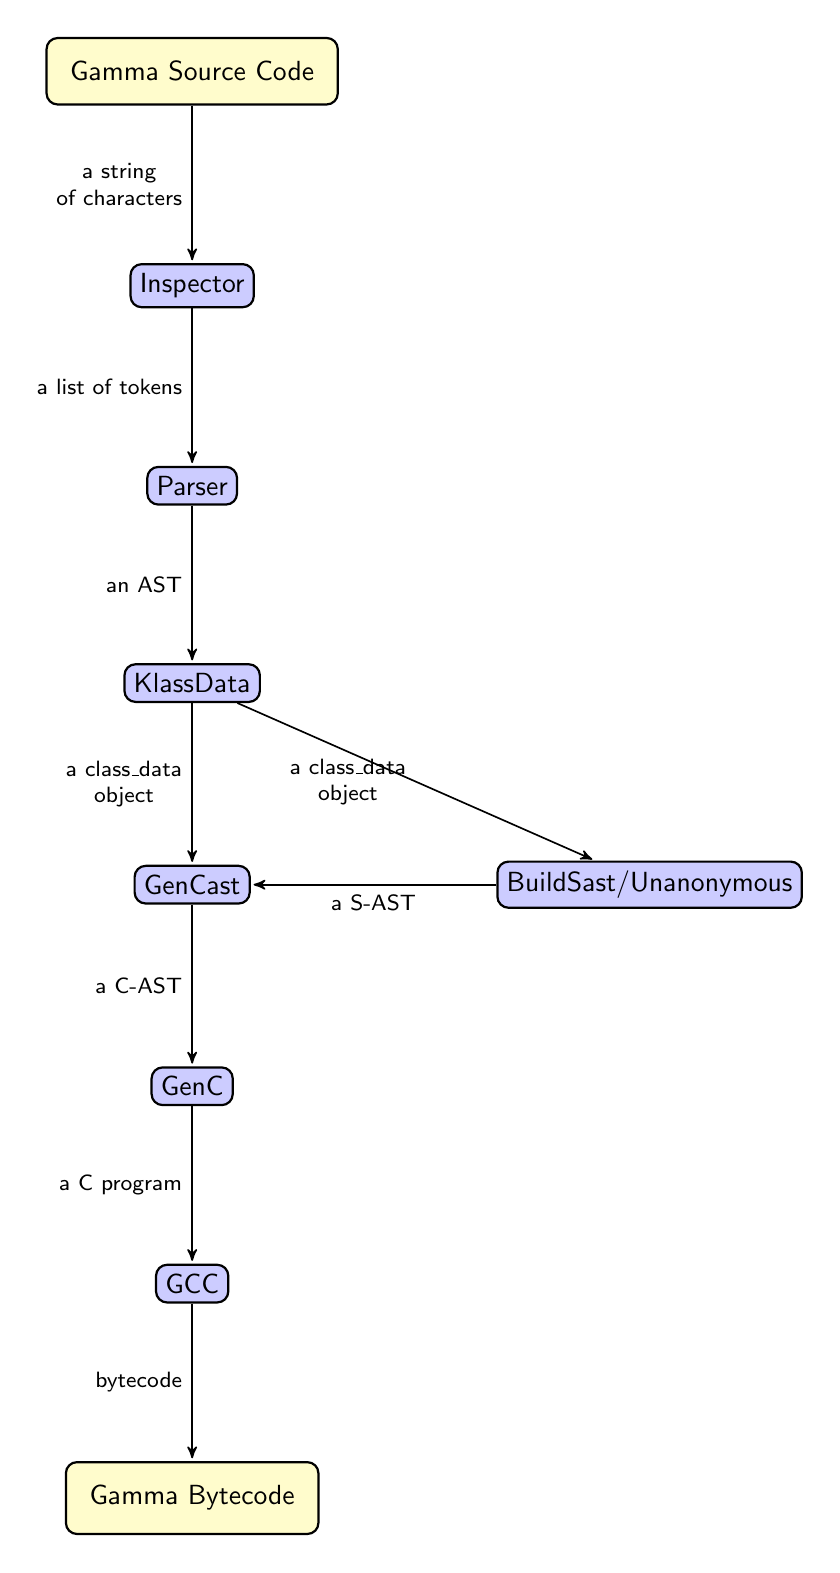
\begin{tikzpicture}[
  font=\sffamily,
  every matrix/.style={ampersand replacement=\&,column sep=2cm,row sep=2cm},
  source/.style={draw,thick,rounded corners,fill=yellow!20,inner sep=.3cm},
  process/.style={draw,thick,rounded corners,fill=blue!20},
  sink/.style={source,fill=green!20},
  dots/.style={gray,scale=2},
  to/.style={->,>=stealth',shorten >=1pt,semithick,font=\sffamily\footnotesize},
  every node/.style={align=center}]

  % Position the nodes using a matrix layout
  \matrix{
    \node[source] (source_code) {Gamma Source Code}; \& \\
    \node[process] (inspect) {Inspector}; \& \\
    \node[process] (parser) {Parser}; \& \\
    \node[process] (klass_data) {KlassData}; \& \\
    \node[process] (gen_cast) {GenCast}; \&
    \node[process] (build_sast) {BuildSast/Unanonymous};\\
    \node[process] (gen_c) {GenC}; \& \\
    \node[process] (gcc) {GCC}; \& \\
    \node[source] (csource) {Gamma Bytecode}; \& \\
  };

  % Draw the arrows between the nodes and label them.
  \draw[to] (source_code) -- node[midway,left] {a string\\of characters} (inspect);
  \draw[to] (inspect) -- node[midway,left] {a list of tokens} (parser);
  \draw[to] (parser) -- node[midway,left] {an AST} (klass_data);
  \draw[to] (klass_data) -- node[midway,left] {a class\_data\\object} (build_sast);
  \draw[to] (klass_data) -- node[midway,left] {a class\_data\\object} (gen_cast);
  \draw[to] (build_sast) -- node[midway,below] {a S-AST} (gen_cast);
  \draw[to] (gen_cast) -- node[midway,left] {a C-AST} (gen_c);
  \draw[to] (gen_c) -- node[midway,left] {a C program} (gcc);
  \draw[to] (gcc) -- node[midway,left] {bytecode} (csource);
\end{tikzpicture}
\end{center}

\subsubsection{Structure by Toplevel Ocaml Function}
\begin{center}
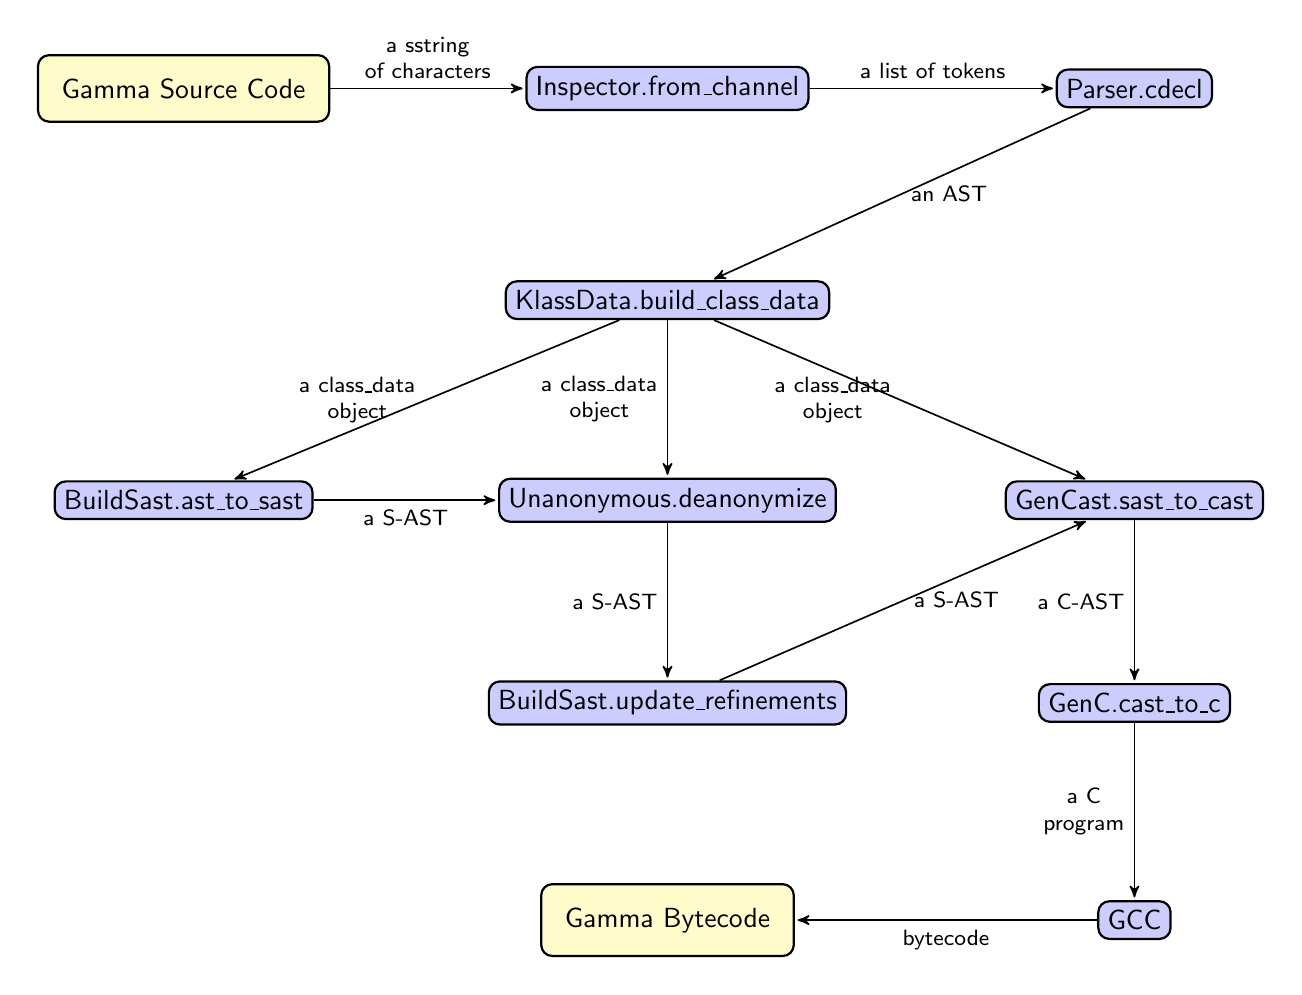
\begin{tikzpicture}[
  font=\sffamily,
  every matrix/.style={ampersand replacement=\&,column sep=2cm,row sep=2cm},
  source/.style={draw,thick,rounded corners,fill=yellow!20,inner sep=.3cm},
  process/.style={draw,thick,rounded corners,fill=blue!20},
  sink/.style={source,fill=green!20},
  dots/.style={gray,scale=2},
  to/.style={->,>=stealth',shorten >=1pt,semithick,font=\sffamily\footnotesize},
  every node/.style={align=center}]

  % Position the nodes using a matrix layout
  \matrix{
    \node[source] (source_code) {Gamma Source Code};\& \node[process] (inspect) {Inspector.from\_channel}; \& \node[process] (parser) {Parser.cdecl}; \\
     \& \node[process] (klass_data) {KlassData.build\_class\_data}; \& \\
     \node[process] (build_sast) {BuildSast.ast\_to\_sast}; \& \node[process] (unam) {Unanonymous.deanonymize}; \& \node[process] (gen_cast) {GenCast.sast\_to\_cast};\\
    \& \node[process] (build_sastr) {BuildSast.update\_refinements}; \& \node[process] (gen_c) {GenC.cast\_to\_c}; \\
    \& \node[source] (csource) {Gamma Bytecode}; \& \node[process] (gcc) {GCC}; \\
  };

  % Draw the arrows between the nodes and label them.
  \draw[to] (source_code) -- node[midway,above] {a sstring\\of characters} (inspect);
  \draw[to] (inspect) -- node[midway,above] {a list of tokens} (parser);
  \draw[to] (parser) -- node[midway,right] {an AST} (klass_data);
  \draw[to] (klass_data) -- node[midway,left] {a class\_data\\object} (build_sast);
  \draw[to] (klass_data) -- node[midway,left] {a class\_data\\object} (unam);
  \draw[to] (klass_data) -- node[midway,left] {a class\_data\\object} (gen_cast);
  \draw[to] (build_sast) -- node[midway,below] {a S-AST} (unam);
  \draw[to] (unam) -- node[midway,left] {a S-AST} (build_sastr);
  \draw[to] (build_sastr) -- node[midway,right] {a S-AST} (gen_cast);
  \draw[to] (gen_cast) -- node[midway,left] {a C-AST} (gen_c);
  \draw[to] (gen_c) -- node[midway,left] {a C\\program} (gcc);
  \draw[to] (gcc) -- node[midway,below] {bytecode} (csource);
\end{tikzpicture}
\end{center}

\subsection{Component Connective Interfaces}
\lstinputlisting[numbers=none,caption=The Main Ray Compiler Ocaml (Trimmed),linerange=19-67]{../../ray/ray.ml}

The primary functionality of the compiler is collected into convenient ocaml modules. From the lexer to the C-AST to C conversion, the connections are the passing of data representations of the current step to the main function of the following module. We utilize as data representations three ASTs (basic, semantic, and C-oriented), a more searchable tabulation of class data, and, of course, a source string and a list of tokens. The presence of Anonymous classes complicates the building of the array of class data and the sast as can be seen by the functor \verb!do_deanom!. Our testing experiences also lead to a more verbose form of AST generation for experimental features, hence \verb!get_data!. In all other cases, the result of the previous step is simply stored in a variable by \verb!let! and passed to the next step. The output of ray is a C file. The user must manually do the final step of compiling this file to bytecode using GCC.

\subsection{Component Authorship}
Each component was a combined effort. This is expressed somewhat in the project role section. However, for clarity, it will be reexpressed in terms of the module archetecture above:

\begin{itemize}
\item Inspector - Weiyuan/Arthy
\item Parser - Ben/Arthy/Matthew
\item KlassData - Matthew
\item Unanonymous - Matthew
\item BuildSast - Matthew/Weiyuan/Arthy
\item GenCast - Matthew/Weiyuan/Ben/Arthy
\item GenC - Matthew/Weiyuan/Ben/Arthy
\item GCC - GNU
\end{itemize}

\section{Test Plan}
\subsection{Examples Gamma Programs}
\subsubsection{Hello World}
This program simply prints "Hello World". It demonstrates the fundamentals needed to write a Gamma program.

\lstinputlisting[caption="Hello World in Gamma"]{../../ray/compiler-tests/programs/helloworld.gamma}

\lstinputlisting[caption="Hello World in Compiled C",language=C]{../../ray/headers/helloworld.c}

\subsubsection{I/O}
This program prompts the user for an integer and a float. It converts the integer to a float and adds the two together. It then prints the equation and result. (You might recognize this from the tutorial.)

\lstinputlisting[caption="I/O in Gamma"]{../../ray/compiler-tests/programs/io.gamma}

\lstinputlisting[caption="I/O in Compiled C",language=C]{../../ray/headers/io.c}

\subsubsection{Argument Reading}
This program prints out each argument passed to the program.

\lstinputlisting[caption="Argument Reading in Gamma"]{../../ray/compiler-tests/programs/args.gamma}

\lstinputlisting[caption="Argument Reading in Compiled C",language=C]{../../ray/headers/args.c}


\begin{itemize}
\item {\bf Arthy}\\
First of all, I should thank my wonderful team mates and I enjoyed every bit working with them. Be it clearly silly
questions on the language or design or OCAML anything and everything they were always there! And without them it would
have certainly not been possible to have pulled this project i must confess well yea at the last moment. Thanks guys!

Thanks to Professor Edwards for making this course so much fun - you never feel the pressure of taking a theoretical course as this - as he puts it - "...in how many other theoretical courses have you had a lecture that ends with a tatooed hand.." 

As any team projects we had our own idiosyncracies that left us with missing deadlines and extending demo deadline and what not - so we were not that one off team which miraculously fit well - we were just like any other team but a team that learnt lessons quickly applied them - left ego outside the door - and worked for the fun of the project! If the team has such a spirit that's all that is required.

DOs and DONTs:
1. Have a team lead 
2. Have one person who is good in OCAML if possible or at least has had experiences with modern programming languages.
3. Have one who is good in programming language theory 
4. Ensure you have team meetings - if people do not turn up or go missing - do open up talk to them 
5. Ensure everyone is comfortable with the project and is at the same pace as yours early on
6. Discuss the design and make a combined decision - different people think differently that definitely will help.
7. This is definitely a fun course and do not spoil it by procastrination - with OCAML you just have few lines to 
code why not start early and get it done early (Smiley)
8. I may want to say do not be ambitious - but in retrospect - I learnt a lot - and may be wish some more - so 
try something cool - after all that's what is grad school for!

Good luck

\item {\bf Ben}\\

\item {\bf Matthew}\\
I had a beginning of an idea of how OOP stuff worked underneath the hood, but this really opened my eyes up to how much work was going on.

It also taught me a lot about making design decisions, and how it's never a good idea to say ``this time we'll just use strings and marker values cause we need it done sooner than later'' -- if Algebraic Data Types are available, use them. Even if it means you 
have to go back and adjust old code because of previous ideas fall out of line with new ones.

I learned how annoying the idea of a NULL value in a typed system can be when we don't give casting as an option (something we should have thought about before), and how smart python is by having methods accept and name the implicit parameter themselves. Good 
job, GvR.

\item {\bf Weiyuan}\\
First I would like to say that this is a very cool, educational and fun project. 

One thing I learned from this project is that I take modern programming languages for granted. I enjoyed many comfortable features and syntactic sugar but never realized there is so much craziness under the hood. We had a long list of ambitious goals at the beginning. Many of them had to be given up as the project went on. From parsing to code generation, I faced a lot of design decisions that I did not even know existed. I gained a much better understanding of how programming languages work and why they are designed the way they are. Also, now I have a completely refreshed view when I see posts titled "Java vs. C++" on the Internet.

Another thing I learned is that proper task division, time management and effective communication are extremely important for a team project. Doing things in parallel and communicating smoothly can save you a lot of trouble.

Finally, I learned my first functional programming language OCaml and I do like it, though I still feel it's weird sometimes.

Advice for future groups:
\begin{itemize}
  \item Start early and procrastinate less
  \item Have a team leader and communicate better
  \item Enjoy it
\end{itemize}

\end{itemize}


\setcounter{lstlisting}{0}

\renewcommand{\lstlistingname}{Source}
\renewcommand{\lstlistlistingname}{Source Files}

\newcommand{\lstsource}[1]{
    \lstinputlisting[caption=\url{#1}]{../../ray/#1}
}
\section{Appendix}
\lstsource{compiler-tests/mix.gamma}
\lstsource{compiler-tests/programs/io.gamma}
\lstsource{compiler-tests/programs/helloworld.gamma}
\lstsource{compiler-tests/programs/args.gamma}
\lstsource{compiler-tests/bad/super-assign.gamma}
\lstsource{compiler-tests/bad/decl.gamma}
\lstsource{compiler-tests/bad/addMix.gamma}
\lstsource{compiler-tests/bad/return1.gamma}
\lstsource{compiler-tests/bad/assign.gamma}
\lstsource{compiler-tests/bad/static.gamma}
\lstsource{compiler-tests/bad/refine_refinable.gamma}
\lstsource{compiler-tests/bad/return2.gamma}
\lstsource{compiler-tests/bad/return3.gamma}
\lstsource{compiler-tests/bad/refinable.gamma}
\lstsource{compiler-tests/stmts/while_condn.gamma}
\lstsource{compiler-tests/stmts/while.gamma}
\lstsource{compiler-tests/stmts/if.gamma}
\lstsource{compiler-tests/exprs/addInt.gamma}
\lstsource{compiler-tests/exprs/prod.gamma}
\lstsource{compiler-tests/exprs/subMix.gamma}
\lstsource{compiler-tests/exprs/super-assign.gamma}
\lstsource{compiler-tests/exprs/divMix.gamma}
\lstsource{compiler-tests/exprs/addMix.gamma}
\lstsource{compiler-tests/exprs/ifeq.gamma}
\lstsource{compiler-tests/exprs/mod.gamma}
\lstsource{compiler-tests/exprs/anonymous.gamma}
\lstsource{compiler-tests/exprs/powMix.gamma}
\lstsource{compiler-tests/exprs/prodMix.gamma}
\lstsource{compiler-tests/exprs/simple-refine.gamma}
\lstsource{compiler-tests/exprs/newarr.gamma}
\lstsource{compiler-tests/exprs/addFloat.gamma}
\lstsource{compiler-tests/exprs/div.gamma}
\lstsource{compiler-tests/exprs/refine_refinable.gamma}
\lstsource{compiler-tests/exprs/refinable.gamma}
\lstsource{compiler-tests/structure/main.gamma}
\lstsource{compiler-tests/structure/no-bodies.gamma}
\lstsource{compiler-tests/structure/func.gamma}
\lstsource{Debug.ml}
\lstsource{ray.ml}
\lstsource{unittest/bkup.ml}
\lstsource{unittest/sast.ml}
\lstsource{parser.mly}
\lstsource{Klass.ml}
\lstsource{Makefile}
\lstsource{BuildSast.mli}
\lstsource{demo/nqueens.gamma}
\lstsource{demo/helloworld.gamma}
\lstsource{demo/bank.gamma}
\lstsource{WhiteSpace.ml}
\lstsource{GenC.ml}
\lstsource{freevars.ml}
\lstsource{streams.ml}
\lstsource{BuiltIns.mli}
\lstsource{canonical.ml}
\lstsource{GlobalData.mli}
\lstsource{scanner.mll}
\lstsource{BuildSast.ml}
\lstsource{Ast.mli}
\lstsource{prettify.ml}
\lstsource{Unanonymous.mli}
\lstsource{headers/gamma-builtin-functions.h}
\lstsource{headers/gamma-builtin-meta.h}
\lstsource{headers/gamma-builtin-struct.h}
\lstsource{headers/gamma-preamble.h}
\lstsource{Sast.mli}
\lstsource{Cast.mli}
\lstsource{run-compiler-test.sh}
\lstsource{Util.ml}
\lstsource{Inspector.ml}
\lstsource{StringModules.ml}
\lstsource{Inspector.mli}
\lstsource{inspect.ml}
\lstsource{Pretty.ml}
\lstsource{UID.ml}
\lstsource{tools/show-example}
\lstsource{tools/runtool}
\lstsource{GenCast.ml}
\lstsource{Klass.mli}
\lstsource{BuiltIns.ml}
\lstsource{Variables.ml}
\lstsource{ctest/compile}
\lstsource{classinfo.ml}
\lstsource{test/parser}
\lstsource{test/README}
\lstsource{test/.testdrive}
\lstsource{test/ast-pretty}
\lstsource{test/scanner}
\lstsource{test/tests/Brace/Empty/Class}
\lstsource{test/tests/Brace/Empty/InitMethod}
\lstsource{test/tests/Brace/Empty/Refinements}
\lstsource{test/tests/Brace/Empty/Method}
\lstsource{test/tests/Brace/Empty/Private}
\lstsource{test/tests/Brace/Empty/WhileMethod}
\lstsource{test/tests/Brace/Empty/Init}
\lstsource{test/tests/Brace/Empty/Public}
\lstsource{test/tests/Brace/Empty/Protected}
\lstsource{test/tests/Brace/Empty/IfMethod}
\lstsource{test/tests/Brace/Multi/Collection}
\lstsource{test/tests/Brace/Trivial/InitStatement}
\lstsource{test/tests/Brace/Trivial/MainWithBuilding}
\lstsource{test/tests/Brace/Simple/Rectangle}
\lstsource{test/tests/Mixed1/Empty/Class}
\lstsource{test/tests/Mixed1/Empty/InitMethod}
\lstsource{test/tests/Mixed1/Empty/Refinements}
\lstsource{test/tests/Mixed1/Empty/Method}
\lstsource{test/tests/Mixed1/Empty/Private}
\lstsource{test/tests/Mixed1/Empty/WhileMethod}
\lstsource{test/tests/Mixed1/Empty/Init}
\lstsource{test/tests/Mixed1/Empty/Public}
\lstsource{test/tests/Mixed1/Empty/Protected}
\lstsource{test/tests/Mixed1/Empty/IfMethod}
\lstsource{test/tests/Mixed1/Multi/Collection}
\lstsource{test/tests/Mixed1/Trivial/InitStatement}
\lstsource{test/tests/Mixed1/Simple/Rectangle}
\lstsource{test/tests/Space/Empty/Class}
\lstsource{test/tests/Space/Empty/InitMethod}
\lstsource{test/tests/Space/Empty/Refinements}
\lstsource{test/tests/Space/Empty/Method}
\lstsource{test/tests/Space/Empty/Private}
\lstsource{test/tests/Space/Empty/WhileMethod}
\lstsource{test/tests/Space/Empty/Init}
\lstsource{test/tests/Space/Empty/Public}
\lstsource{test/tests/Space/Empty/Protected}
\lstsource{test/tests/Space/Empty/IfMethod}
\lstsource{test/tests/Space/Multi/Collection}
\lstsource{test/tests/Space/Trivial/InitStatement}
\lstsource{test/tests/Space/Simple/Rectangle}
\lstsource{Unanonymous.ml}
\lstsource{KlassData.mli}
\lstsource{KlassData.ml}


\end{document}